\clearpage
\subsubsection{Sơ đồ luồng dữ liệu DFD}
\label{wispace:sec:dfd}

Phần này trình bày sơ đồ ngữ cảnh và DFD mức 1 của Wispace Speaking, tập trung vào dữ liệu tài khoản, kho đề, bài làm, kết quả và gói dịch vụ. Frontend, backend, hàng đợi và kho dữ liệu thuộc phạm vi hệ thống; các dịch vụ xác thực, TTS, chấm Speaking và thanh toán được xem là tác nhân ngoài.

Luồng dữ liệu được tổ chức quanh các nhóm nghiệp vụ dưới đây. Mã E, P và D chỉ có ý nghĩa trong phạm vi từng hệ thống.

\begin{longtable}{|>{\raggedright\arraybackslash}p{0.07\linewidth}|>{\raggedright\arraybackslash}p{0.25\linewidth}|p{0.58\linewidth}|}
\caption{Tác nhân ngoài của Wispace Speaking}\label{wispace:tab:dfd-entities}\\
\hline
\textbf{Mã} & \textbf{Tác nhân} & \textbf{Dữ liệu trao đổi} \\
\hline
\endfirsthead
\hline
\textbf{Mã} & \textbf{Tác nhân} & \textbf{Dữ liệu trao đổi} \\
\hline
\endhead
E1 & Khách / Học viên & Cung cấp thông tin tài khoản, bộ lọc đề, audio, yêu cầu xem kết quả và thanh toán; nhận nội dung luyện tập, báo cáo và quyền lợi sử dụng. \\
\hline
E2 & Moderator / Admin & Cung cấp dữ liệu đề, quyết định kiểm duyệt, thay đổi người dùng và cấu hình gói; nhận danh sách, trạng thái xử lý và nhật ký. \\
\hline
E3 & Email / Google OAuth & Tiếp nhận nội dung gửi OTP hoặc yêu cầu xác minh Google; trả trạng thái gửi hoặc thông tin danh tính. OTP do người dùng nhập thuộc luồng E1. \\
\hline
E4 & Dịch vụ TTS & Nhận văn bản câu hỏi và lựa chọn giọng; trả audio câu hỏi hoặc thông tin lỗi. \\
\hline
E5 & Scoring Model & Nhận audio và ngữ cảnh câu hỏi; trả transcript, điểm theo tiêu chí, lỗi và nhận xét. \\
\hline
E6 & PayOS & Nhận dữ liệu đơn thanh toán; trả liên kết thanh toán và trạng thái giao dịch đã xác minh. \\
\hline
\end{longtable}


\begin{longtable}{|>{\raggedright\arraybackslash}p{0.07\linewidth}|p{0.48\linewidth}|p{0.35\linewidth}|}
\caption{Tiến trình mức 1 của Wispace Speaking}\label{wispace:tab:dfd-processes}\\
\hline
\textbf{Mã} & \textbf{Tiến trình} & \textbf{Phạm vi} \\
\hline
\endfirsthead
\hline
\textbf{Mã} & \textbf{Tiến trình} & \textbf{Phạm vi} \\
\hline
\endhead
P1 & Xác thực và quản lý hồ sơ & UC01--UC04 \\
\hline
P2 & Tra cứu và quản lý kho đề & UC06--UC08 \\
\hline
P3 & Tiếp nhận bài và chấm Speaking & UC09, UC11 \\
\hline
P4 & Tổng hợp kết quả và tiến bộ & UC10, UC12 \\
\hline
P5 & Quản trị người dùng và gói dịch vụ & UC05; gói dịch vụ ở Chương 5 \\
\hline
\end{longtable}


\begin{longtable}{|>{\raggedright\arraybackslash}p{0.07\linewidth}|p{0.25\linewidth}|p{0.58\linewidth}|}
\caption{Kho dữ liệu của Wispace Speaking}\label{wispace:tab:dfd-stores}\\
\hline
\textbf{Mã} & \textbf{Kho dữ liệu} & \textbf{Nội dung} \\
\hline
\endfirsthead
\hline
\textbf{Mã} & \textbf{Kho dữ liệu} & \textbf{Nội dung} \\
\hline
\endhead
D1 & Tài khoản và phiên & Thông tin tài khoản, hồ sơ, vai trò, trạng thái, OTP và dữ liệu phiên xác thực. \\
\hline
D2 & Kho đề Speaking & Câu hỏi, chủ đề, nguồn đề, trạng thái kiểm duyệt, báo cáo đề và audio câu hỏi. \\
\hline
D3 & Bài làm và kết quả & Phiên luyện tập/thi thử, audio câu trả lời, trạng thái chấm, điểm, transcript, lỗi, tiến bộ và liên kết chia sẻ. \\
\hline
D4 & Gói, quota, thanh toán & Gói dịch vụ, quyền lợi, định mức, bút toán sử dụng/hoàn quota và giao dịch thanh toán. \\
\hline
D5 & Nhật ký quản trị & Người thực hiện, lý do, thời điểm và nội dung thay đổi người dùng hoặc cấu hình gói. \\
\hline
\end{longtable}


\clearpage

\paragraph{Sơ đồ ngữ cảnh.}

Sơ đồ thể hiện toàn bộ Wispace Speaking như một tiến trình duy nhất; các mũi tên ghi rõ dữ liệu gửi đến và dữ liệu trả về cho từng tác nhân ngoài.

\begin{figure}[H]
\centering
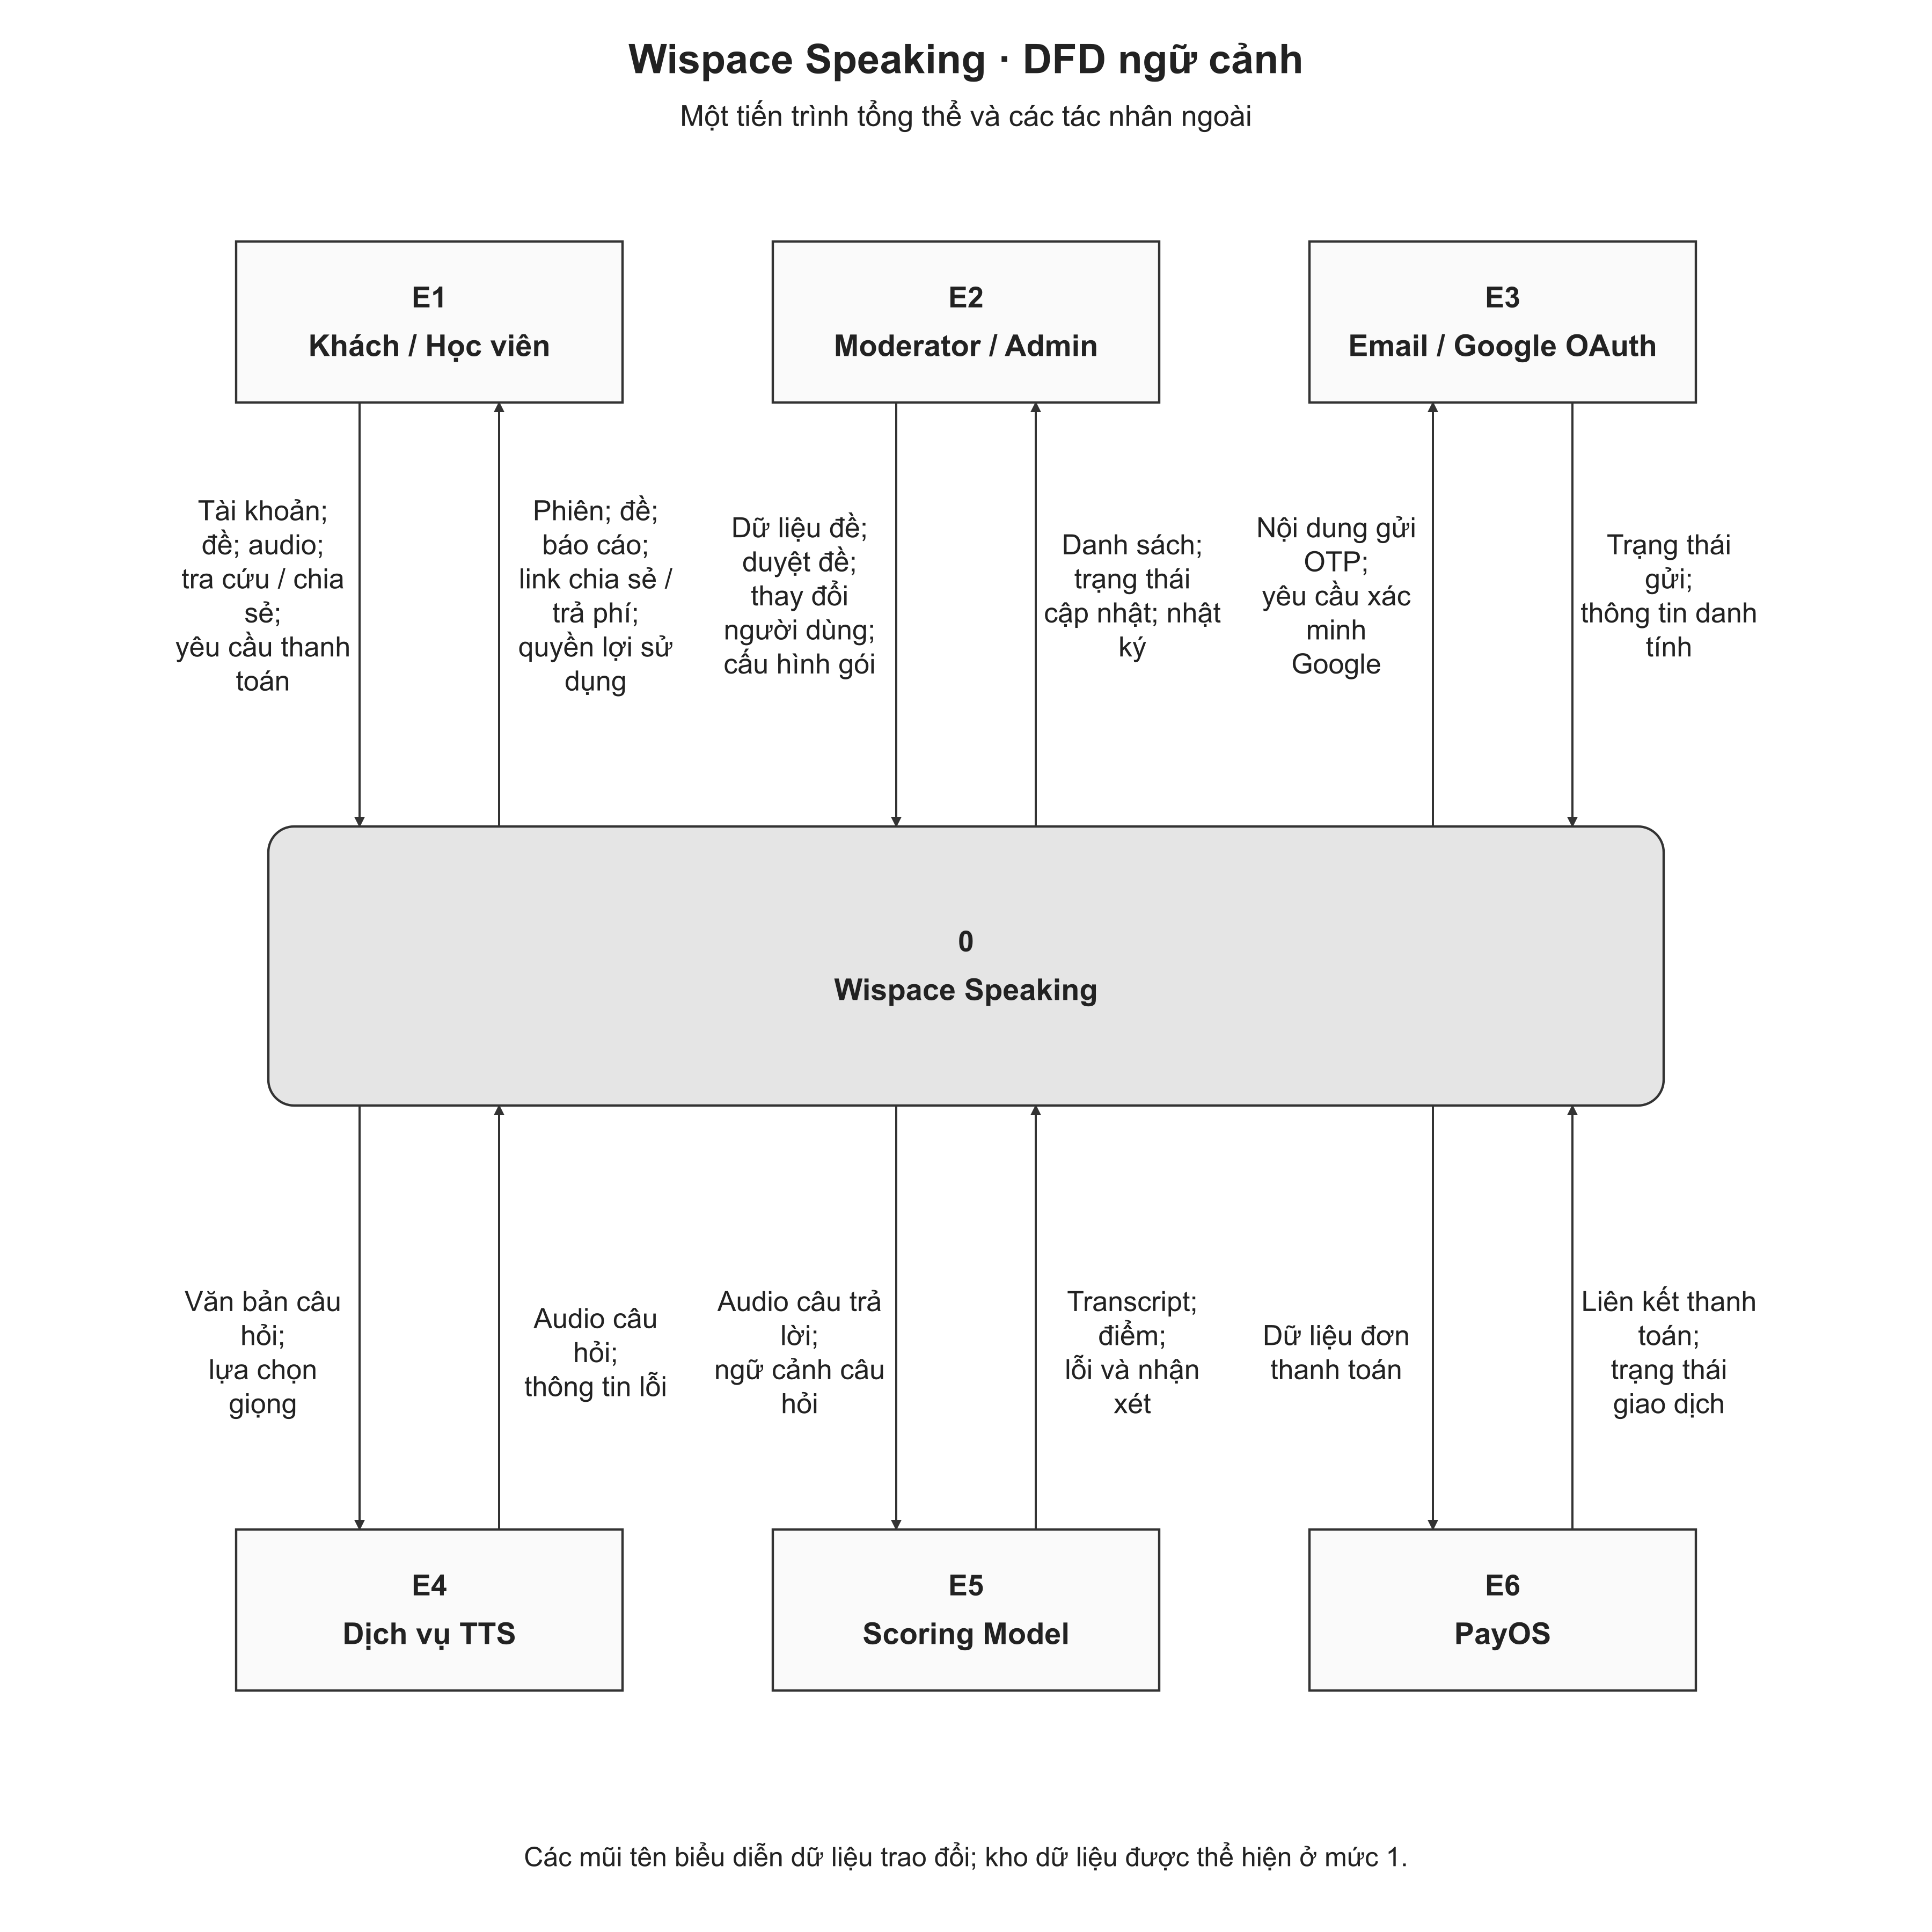
\includegraphics[width=\linewidth,height=0.78\textheight,keepaspectratio]{Images/DFD/Wispace/wispace_dfd_context.png}
\caption{DFD ngữ cảnh của Wispace Speaking}
\label{wispace:fig:dfd-context}
\end{figure}

\clearpage


\paragraph{Sơ đồ mức 1.}

Để giữ nhãn và đường nối dễ đọc, cùng một sơ đồ mức 1 được trình bày thành hai phần. Các tác nhân và kho dữ liệu có cùng mã ở hai phần là cùng một đối tượng logic. Dữ liệu giữa các nhóm xử lý được trao đổi qua kho dùng chung, không phải các bản sao tách biệt.

\clearpage

\begin{figure}[H]
\centering
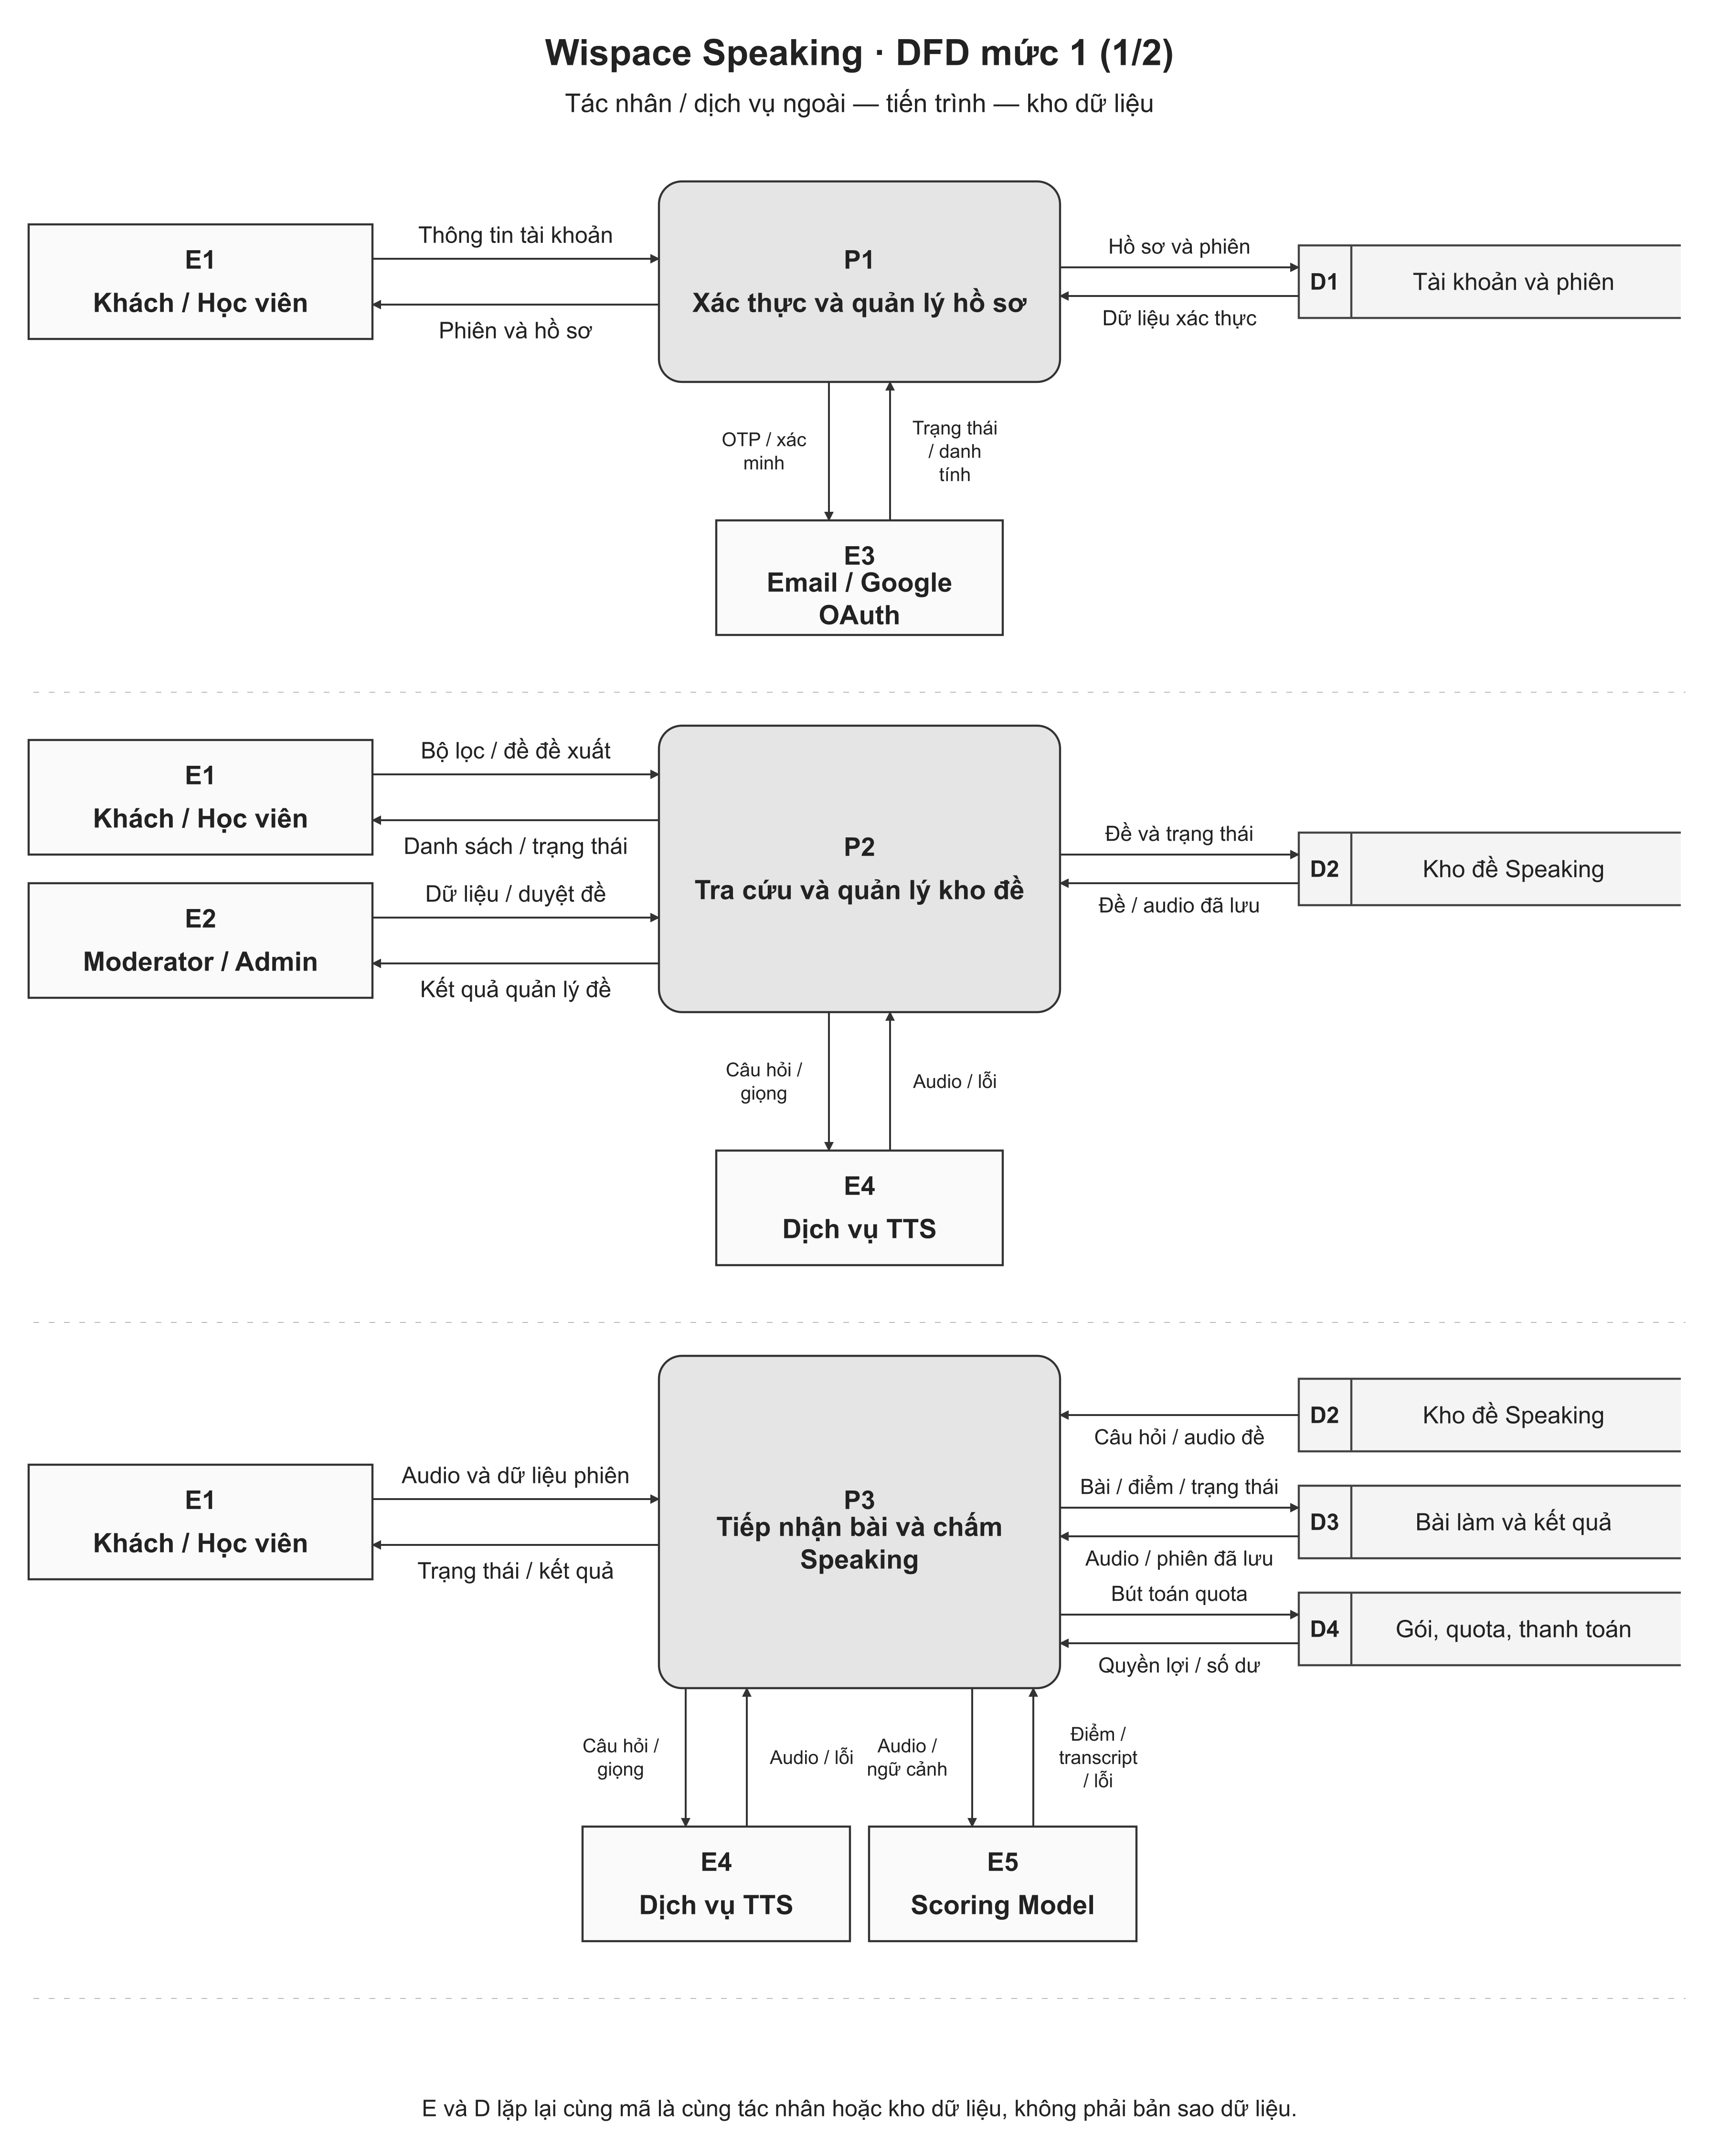
\includegraphics[width=\linewidth,height=0.78\textheight,keepaspectratio]{Images/DFD/Wispace/wispace_dfd_level1_1.png}
\caption{DFD mức 1 của Wispace Speaking: P1, P2, P3}
\label{wispace:fig:dfd-level1-1}
\end{figure}

\clearpage

\begin{figure}[H]
\centering
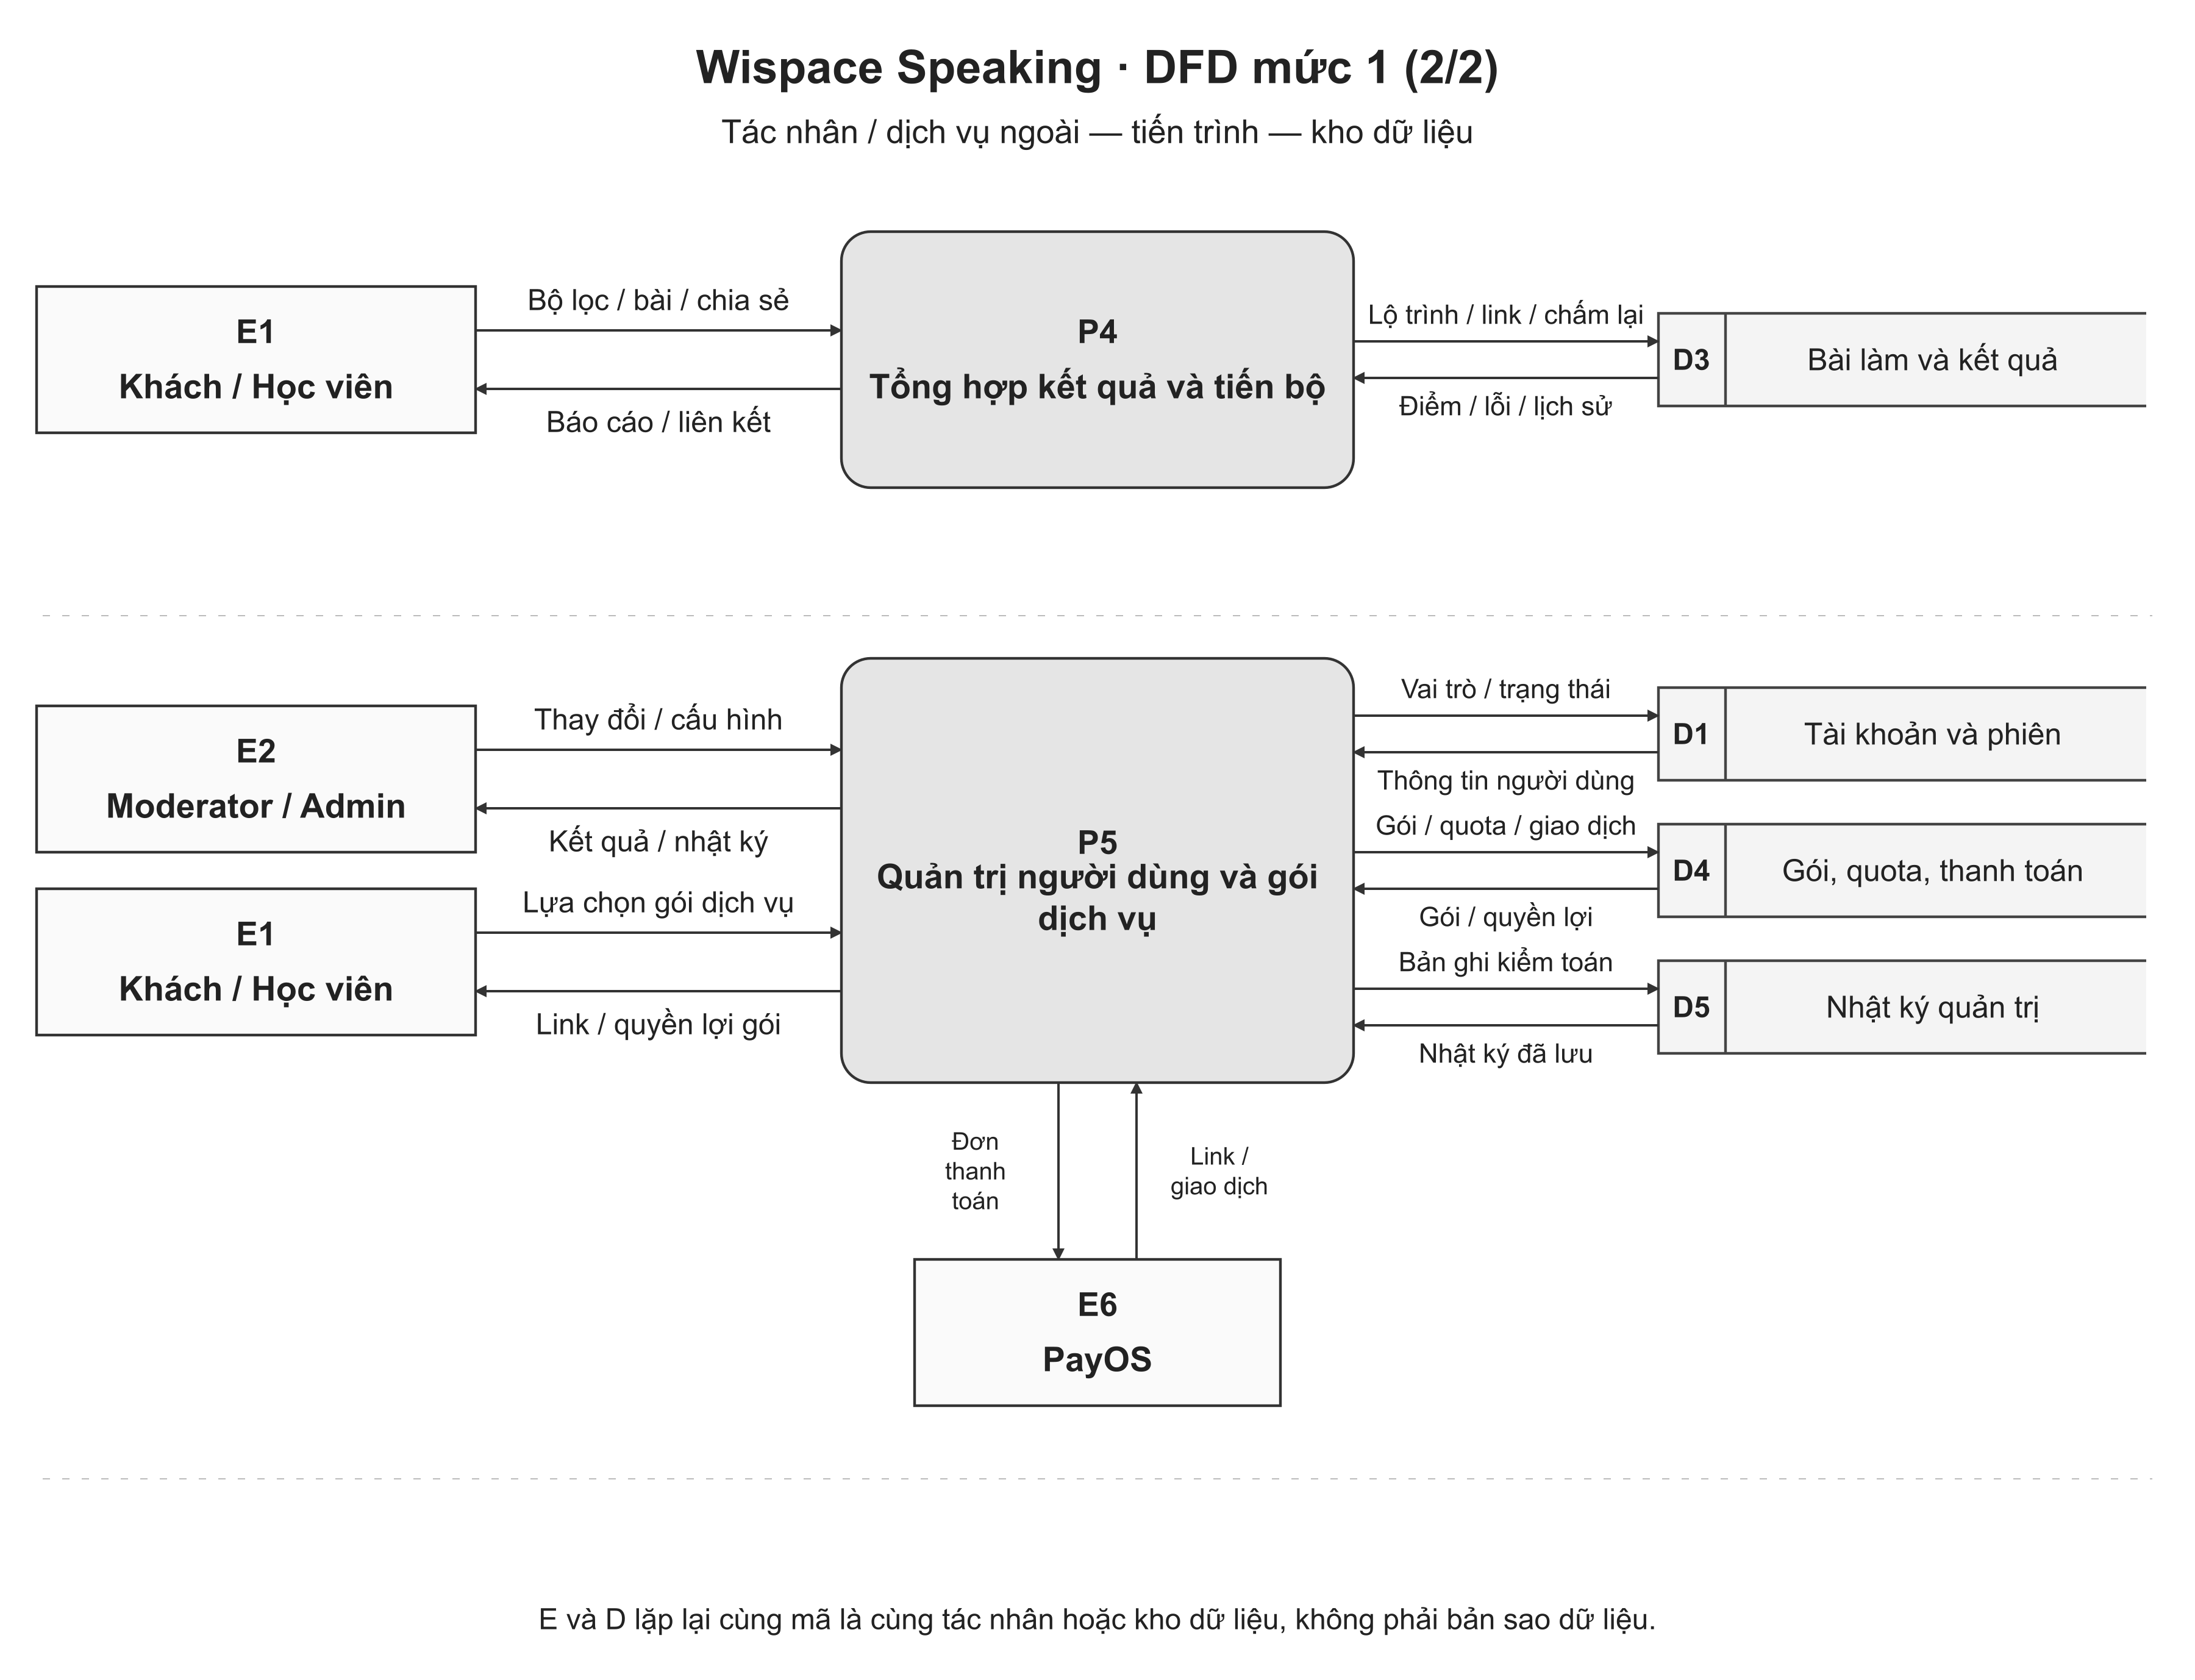
\includegraphics[width=\linewidth,height=0.78\textheight,keepaspectratio]{Images/DFD/Wispace/wispace_dfd_level1_2.png}
\caption{DFD mức 1 của Wispace Speaking: P4, P5}
\label{wispace:fig:dfd-level1-2}
\end{figure}




P3 đọc câu hỏi từ D2, ghi audio và kết quả vào D3, đồng thời cập nhật bút toán quota ở D4. P4 dùng dữ liệu D3 để lập báo cáo, thống kê tiến bộ và quản lý liên kết chia sẻ; yêu cầu chấm lại được ghi vào trạng thái bài làm ở D3 để P3 xử lý. P5 bao gồm yêu cầu mua gói đã nêu ở Chương 5, ngoài phạm vi 12 use-case chi tiết.
